\section{Vehicle Stop Frequency}
\label{sec:Results_Stops}

Vehicle–stop frequency is the natural kinematic counterpart to the mean‐speed metric discussed in Section~\ref{sec:Results_MeanSpeed}: every time the platoon’s mean speed falls, an accompanying rise in complete halts is expected. Table~\ref{tab:StopFreq} and Figures~\ref{fig:StopFreq_2077}–\ref{fig:StopFreq_3462} therefore replicate the structure of the previous section, yet emphasise discrete stop events rather than continuous velocity.

\subparagraph*{General behaviour.}
For light and moderate flows ($69$–$1385\,\mathrm{veh/h}$) both \ac{eco-glosa} and \ac{flow-glosa} \emph{decrease} stops monotonically with higher \ac{mpr}. At $138\,\mathrm{veh/h}$, HBEFA4–\ac{eco-glosa} cuts stops from \textbf{0.83} to $0.08$\,stops/veh at $90\,\%$ \ac{mpr} (Figure~\ref{fig:StopFreq_2077}a), a $90\,\%$ reduction. \ac{flow-glosa} achieves a similar reduction but typically needs about $10$\,pp more penetration, consistent with its slightly higher cruise speeds.

\subparagraph*{2077\,veh/h --- incipient congestion.}
Figure~\ref{fig:StopFreq_2077} illustrates that vehicle stops begin at approximately $1.06$\,stops/veh in the Standard case. Under the PHEMlight5 emission model, \ac{eco-glosa} initially records a slight increase to \textbf{$1.08$}\,stops/veh at $10\,\%$\,\ac{mpr}, indicative of emerging congestion. In contrast, under HBEFA4, \ac{eco-glosa} decreases to $1.03$\,stops/veh before continuing downward consistently. \ac{flow-glosa} already lowers stops to $0.99$\,stops/veh at $10\,\%$ and practically eliminates them ($0.03$\,stops/veh) by $90\,\%$, demonstrating strong queue-suppression just below the jam threshold.

\subparagraph*{2769\,veh/h --- jam threshold.}
Figure~\ref{fig:StopFreq_2769} highlights significant divergence between the two emission models. Under PHEMlight5, the stop frequency for \ac{eco-glosa} increases sharply from \textbf{$1.36$}\,stops/veh (Standard) to \textbf{$9.53$}\,stops/veh at $20\,\%$\,\ac{mpr}, ultimately peaking at \textbf{$23.11$}\,stops/veh by $90\,\%$\,\ac{mpr}. The HBEFA4-based \ac{eco-glosa} exhibits a similar, albeit delayed, trend: it remains around $1.47$\,stops/veh at $10\,\%$\,\ac{mpr}, before rapidly escalating to \textbf{$7.74$}\,stops/veh at $30\,\%$ and reaching as high as \textbf{$16.04$}\,stops/veh at $60\,\%$. Throughout, \ac{flow-glosa} remains below $1.28$\,stops/veh and declines smoothly to $0.07$\,stops/veh at $90\,\%$, showing robust wave-dampening at the verge of congestion.

\subparagraph*{3462\,veh/h --- full saturation.}
Figure~\ref{fig:StopFreq_3462} shows that all evaluated algorithms enter a fully saturated (gridlocked) state at a demand of $3462\,\mathrm{veh/h}$. Under HBEFA4, \ac{eco-glosa} exhibits a monotonic increase in stops, peaking at \textbf{$35.14$}\,stops/veh at $80\,\%$\,\ac{mpr}. Similarly, PHEMlight5-based \ac{eco-glosa} reaches an even higher maximum of \textbf{$38.94$}\,stops/veh at $100\,\%$\,\ac{mpr}. In stark contrast, \ac{flow-glosa} sharply reduces stops beyond $50\%$ \ac{mpr}, dropping to $5.28$\,stops/veh at $60\%$, then falling to near zero ($0.19$ at $80\%$, $0.01$ at $90\%$, $0.00$ at $100\%$), indicative of a dissolved queue rather than a perpetual standstill. Simultaneously, mean speeds under \ac{flow-glosa} climb well above the jam threshold of $4\,\mathrm{m/s}$ (Figures~\ref{fig:MeanSpeed_HBEFA4_3462} and~\ref{fig:MeanSpeed_PHEM_3462}), confirming that the advisory successfully restores free‐flow conditions once a critical penetration is reached. Thus, at extreme demand, \ac{flow-glosa} not only prevents further stops but actively resolves the gridlock, demonstrating its capacity to recover throughput under severe saturation.

\subparagraph*{Key takeaways.}
\begin{enumerate}[label=(\alph*)]
  \item For light to moderate demand ($69$–$1385\,\mathrm{veh/h}$), both \ac{eco-glosa} and \ac{flow-glosa} monotonically reduce stop frequency as \ac{mpr} rises; \ac{eco-glosa} achieves the lowest counts at high penetration (e.g.\ a 90\% reduction at $138\,\mathrm{veh/h}$).
  \item At incipient congestion ($2077\,\mathrm{veh/h}$), \ac{flow-glosa} suppresses stops most effectively, driving them below $0.1$\,stops/veh at $90\%$ \ac{mpr}, whereas \ac{eco-glosa} under PHEMlight5 briefly increases stops at low penetration before eventual decline.
  \item At the jam threshold ($2769\,\mathrm{veh/h}$), \ac{eco-glosa} experiences runaway stop counts (exceeding 20\,stops/veh), with PHEMlight5 amplifying the effect; \ac{flow-glosa}, in contrast, keeps stops below $1.3$\,stops/veh and continues to decline with \ac{mpr}.
  \item Under full saturation ($3462\,\mathrm{veh/h}$), only \ac{flow-glosa} dissolves the queue beyond 80\% \ac{mpr}, driving stop counts to near zero and restoring mean speeds above $4\,\mathrm{m/s}$, whereas \ac{eco-glosa} accumulates over 35\,stops/veh.
  \item A combined assessment of stop-frequency and speed metrics is essential: joint interpretation distinguishes true gridlock resolution under \ac{flow-glosa} from \enquote{false zero} stops when vehicles remain immobilised.
\end{enumerate}

\begin{figure}[htb]
  \centering
  \begin{subfigure}[b]{0.45\textwidth}
    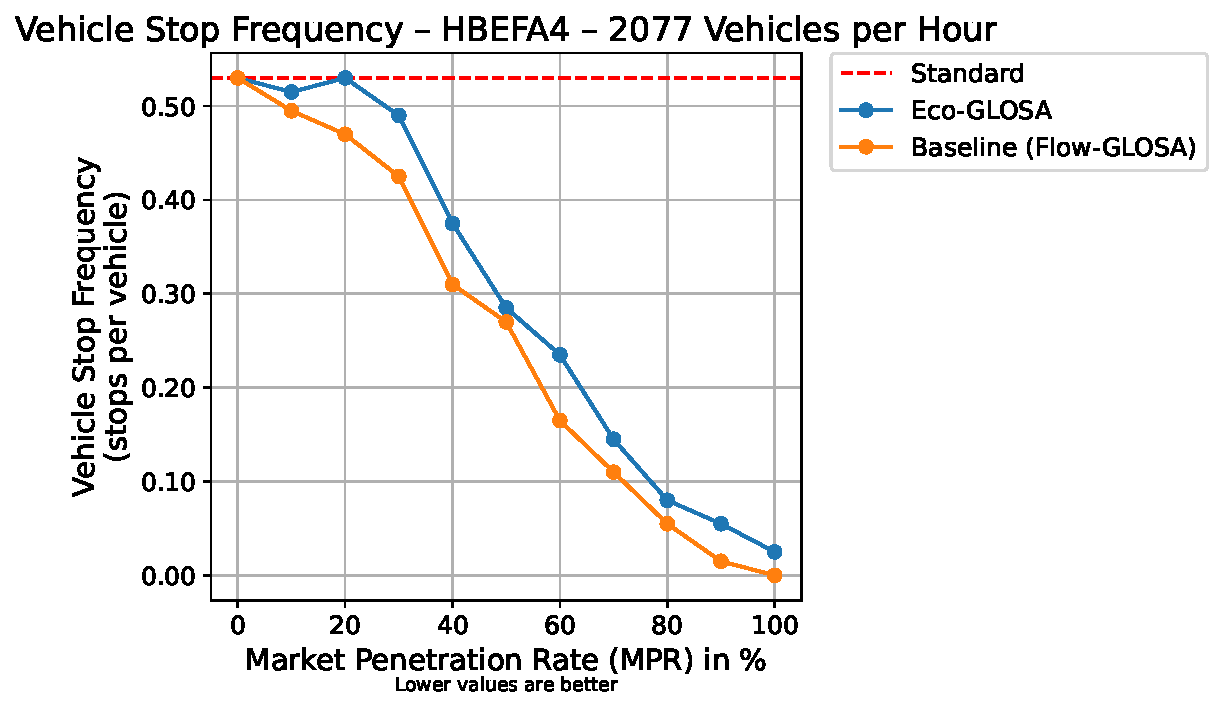
\includegraphics[width=\textwidth]{data/img/VehicleStopFrequency/VehicleStopFrequency_HBEFA4_Cars2077.pdf}
    \caption{Vehicle stop frequency versus \ac{mpr} for the HBEFA4 emission model at $2077\,\mathrm{veh/h}$.}
  \end{subfigure}\hfill
  \begin{subfigure}[b]{0.45\textwidth}
    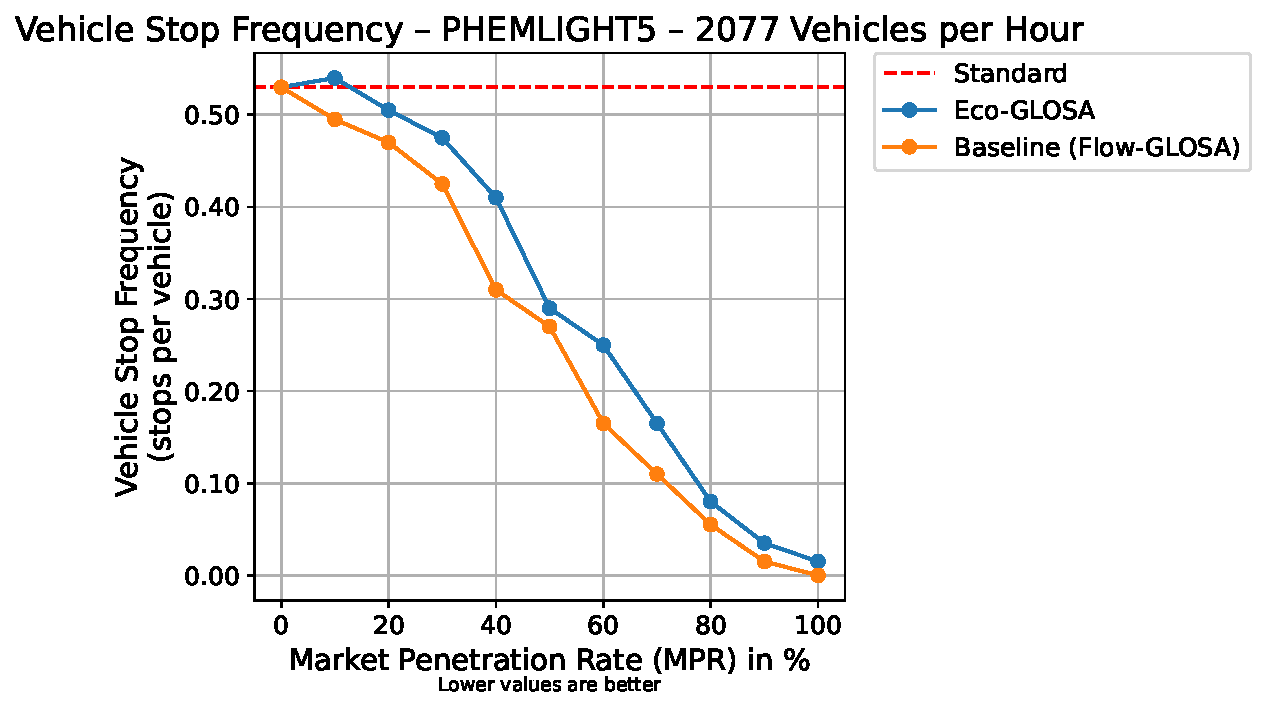
\includegraphics[width=\textwidth]{data/img/VehicleStopFrequency/VehicleStopFrequency_PHEMLIGHT5_Cars2077.pdf}
    \caption{Vehicle stop frequency versus \ac{mpr} for the PHEMlight5 emission model at $2077\,\mathrm{veh/h}$.}
  \end{subfigure}
  \caption{Vehicle stop frequency as a function of \ac{mpr} at a traffic volume of $2077\,\mathrm{veh/h}$, comparing Standard, \ac{eco-glosa}, and \ac{flow-glosa} algorithms.}
  \label{fig:StopFreq_2077}
\end{figure}

\begin{figure}[htb]
  \centering
  \begin{subfigure}[b]{0.45\textwidth}
    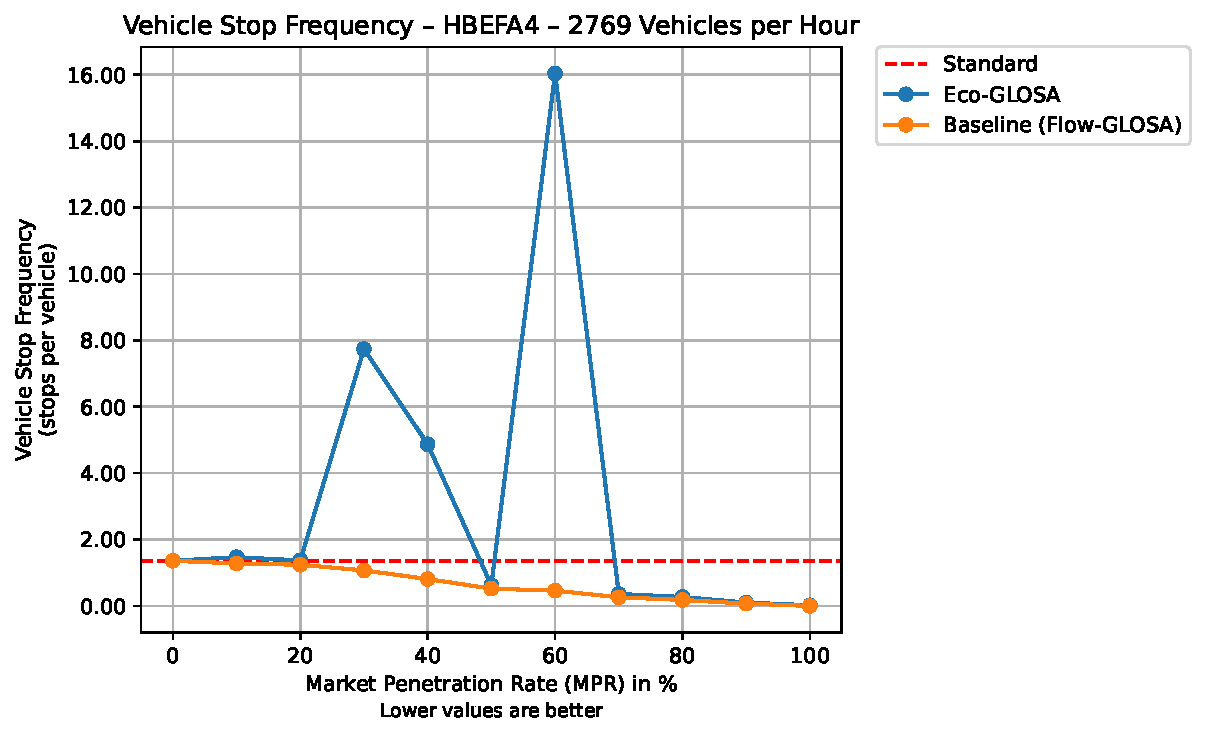
\includegraphics[width=\textwidth]{data/img/VehicleStopFrequency/VehicleStopFrequency_HBEFA4_Cars2769.pdf}
    \caption{Vehicle stop frequency versus \ac{mpr} for the HBEFA4 emission model at $2769\,\mathrm{veh/h}$.}
  \end{subfigure}\hfill
  \begin{subfigure}[b]{0.45\textwidth}
    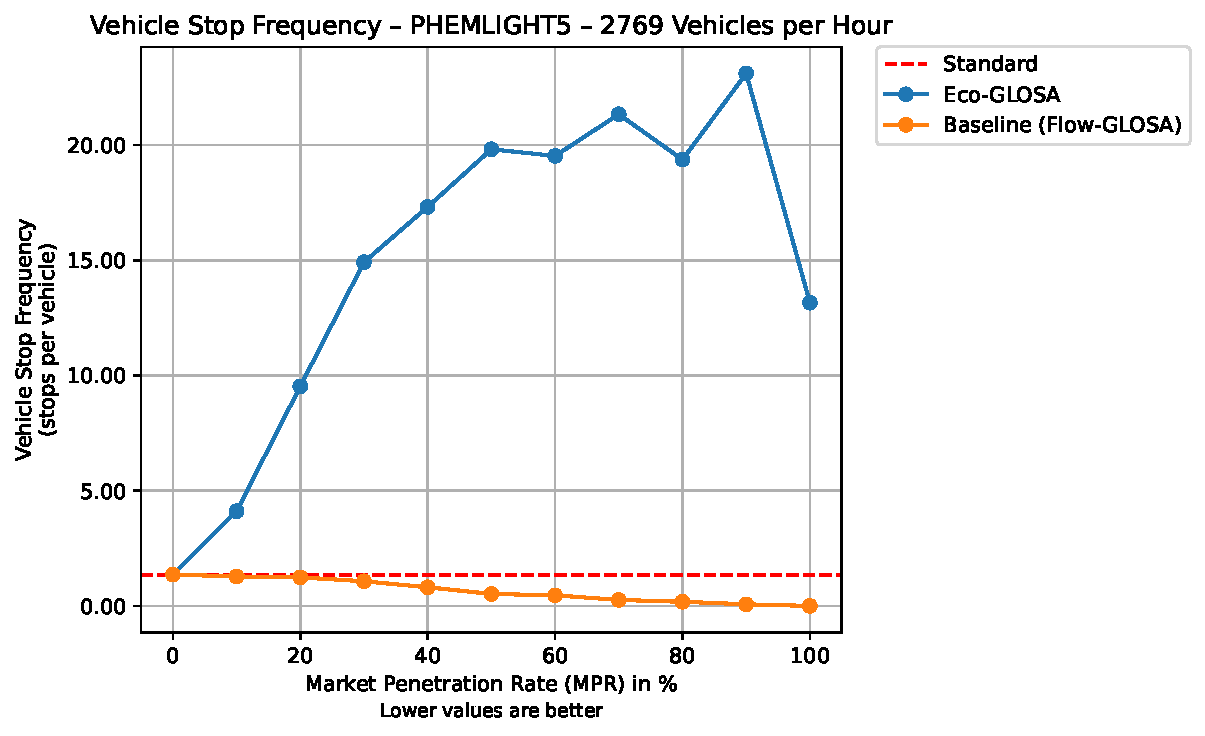
\includegraphics[width=\textwidth]{data/img/VehicleStopFrequency/VehicleStopFrequency_PHEMLIGHT5_Cars2769.pdf}
    \caption{Vehicle stop frequency versus \ac{mpr} for the PHEMlight5 emission model at $2769\,\mathrm{veh/h}$.}
  \end{subfigure}
  \caption{Vehicle stop frequency as a function of \ac{mpr} at a traffic volume of $2769\,\mathrm{veh/h}$, comparing Standard, \ac{eco-glosa}, and \ac{flow-glosa} algorithms.}
  \label{fig:StopFreq_2769}
\end{figure}

\begin{figure}[htb]
  \centering
  \begin{subfigure}[b]{0.45\textwidth}
    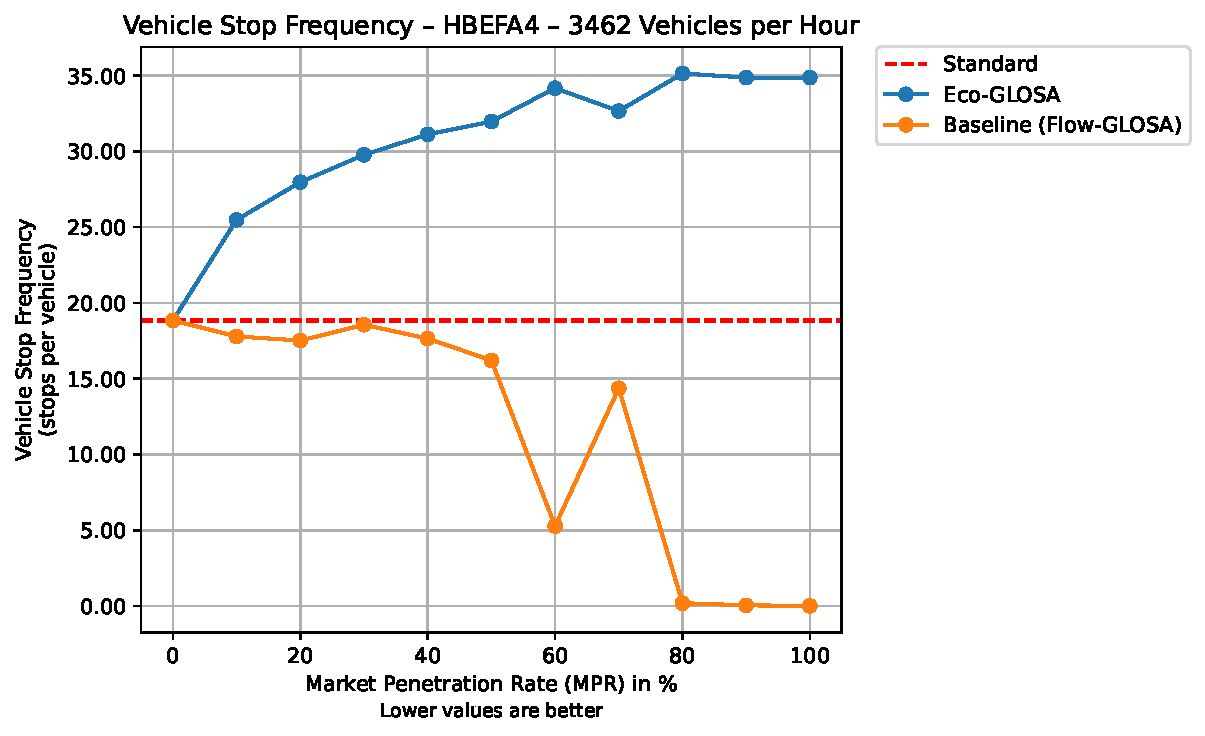
\includegraphics[width=\textwidth]{data/img/VehicleStopFrequency/VehicleStopFrequency_HBEFA4_Cars3462.pdf}
    \caption{Vehicle stop frequency versus \ac{mpr} for the HBEFA4 emission model at $3462\,\mathrm{veh/h}$.}
  \end{subfigure}\hfill
  \begin{subfigure}[b]{0.45\textwidth}
    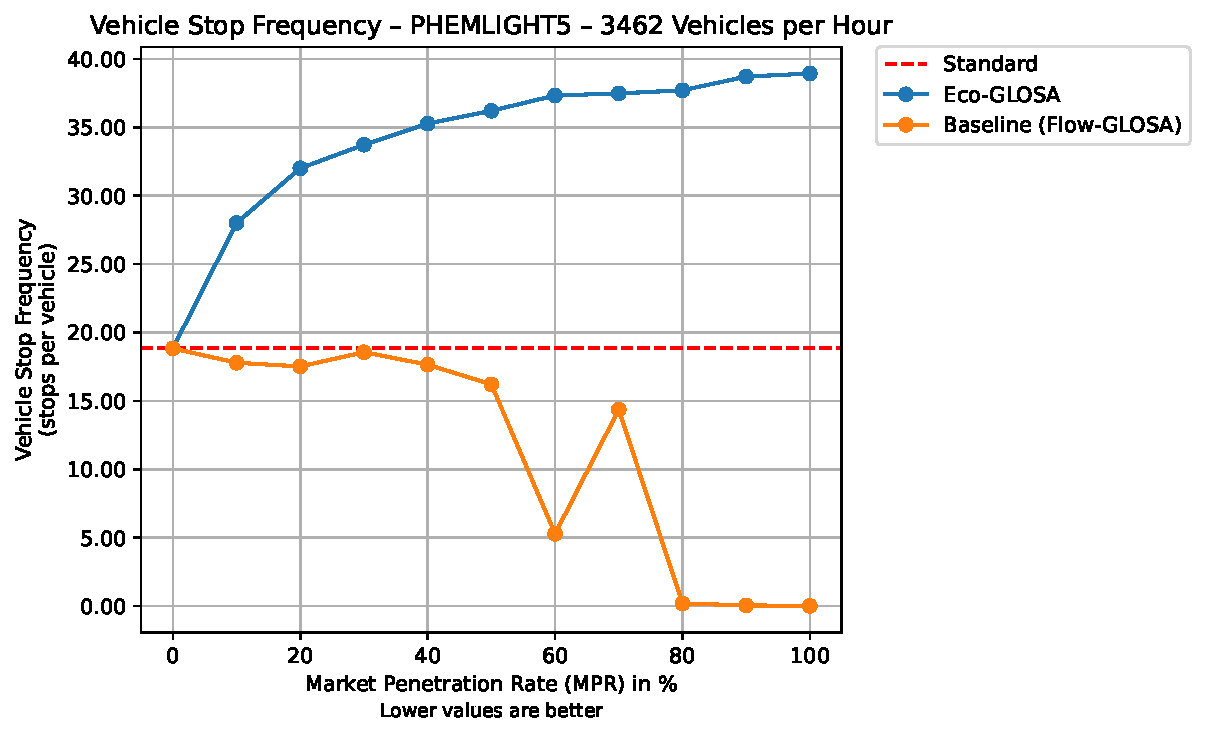
\includegraphics[width=\textwidth]{data/img/VehicleStopFrequency/VehicleStopFrequency_PHEMLIGHT5_Cars3462.pdf}
    \caption{Vehicle stop frequency versus \ac{mpr} for the PHEMlight5 emission model at $3462\,\mathrm{veh/h}$.}
  \end{subfigure}
  \caption{Vehicle stop frequency as a function of \ac{mpr} at a traffic volume of $3462\,\mathrm{veh/h}$, comparing Standard, \ac{eco-glosa}, and \ac{flow-glosa} algorithms.}
  \label{fig:StopFreq_3462}
\end{figure}


\begin{table}[htb]
  \centering
  \caption{Vehicle stop frequency, expressed as average stops per vehicle, for various traffic volumes and \acp{mpr}. Results are provided for the Standard (no \ac{glosa}), \ac{flow-glosa}, and \ac{eco-glosa} configurations under the HBEFA4 and PHEMlight5 emission models.}
  \label{tab:StopFreq}
  \resizebox{\textwidth}{!}{%
  \begin{tabular}{r l l r *{10}{r}}
    \toprule
    Cars & Algorithm & Fuel Model & \textbf{0\% (Standard)} & 10\% & 20\% & 30\% & 40\% & 50\% & 60\% & 70\% & 80\% & 90\% & 100\%\\
    \midrule
    69  & \ac{eco-glosa} & HBEFA4 & \textbf{0.76} & 0.56 & 0.72 & 0.56 & 0.49 & 0.54 & 0.43 & 0.22 & 0.28 & 0.11 & 0.00\\
    69  & Baseline (\ac{flow-glosa}) & HBEFA4 & \textbf{0.76} & 0.56 & 0.78 & 0.61 & 0.49 & 0.54 & 0.49 & 0.22 & 0.28 & 0.17 & 0.00\\
    69  & \ac{eco-glosa} & PHEMLIGHT5 & \textbf{0.76} & 0.56 & 0.72 & 0.50 & 0.49 & 0.54 & 0.43 & 0.22 & 0.28 & 0.11 & 0.00\\
    69  & Baseline (\ac{flow-glosa}) & PHEMLIGHT5 & \textbf{0.76} & 0.56 & 0.78 & 0.61 & 0.49 & 0.54 & 0.49 & 0.22 & 0.28 & 0.17 & 0.00\\
    \midrule
    138 & \ac{eco-glosa} & HBEFA4 & \textbf{0.83} & 0.64 & 0.64 & 0.59 & 0.37 & 0.27 & 0.27 & 0.19 & 0.13 & 0.08 & 0.00\\
    138 & Baseline (\ac{flow-glosa}) & HBEFA4 & \textbf{0.83} & 0.61 & 0.62 & 0.59 & 0.37 & 0.32 & 0.24 & 0.16 & 0.16 & 0.05 & 0.00\\
    138 & \ac{eco-glosa} & PHEMLIGHT5 & \textbf{0.83} & 0.67 & 0.56 & 0.59 & 0.37 & 0.29 & 0.16 & 0.19 & 0.13 & 0.08 & 0.00\\
    138 & Baseline (\ac{flow-glosa}) & PHEMLIGHT5 & \textbf{0.83} & 0.61 & 0.62 & 0.59 & 0.37 & 0.32 & 0.24 & 0.16 & 0.16 & 0.05 & 0.00\\
    \midrule
    346 & \ac{eco-glosa} & HBEFA4 & \textbf{0.76} & 0.68 & 0.65 & 0.51 & 0.47 & 0.38 & 0.28 & 0.27 & 0.19 & 0.08 & 0.01\\
    346 & Baseline (\ac{flow-glosa}) & HBEFA4 & \textbf{0.76} & 0.69 & 0.64 & 0.49 & 0.44 & 0.36 & 0.24 & 0.27 & 0.15 & 0.06 & 0.00\\
    346 & \ac{eco-glosa} & PHEMLIGHT5 & \textbf{0.76} & 0.65 & 0.73 & 0.56 & 0.51 & 0.35 & 0.31 & 0.27 & 0.17 & 0.07 & 0.03\\
    346 & Baseline (\ac{flow-glosa}) & PHEMLIGHT5 & \textbf{0.76} & 0.69 & 0.64 & 0.49 & 0.44 & 0.36 & 0.24 & 0.27 & 0.15 & 0.06 & 0.00\\
    \midrule
    692 & \ac{eco-glosa} & HBEFA4 & \textbf{0.79} & 0.78 & 0.62 & 0.54 & 0.45 & 0.42 & 0.23 & 0.26 & 0.16 & 0.06 & 0.01\\
    692 & Baseline (\ac{flow-glosa}) & HBEFA4 & \textbf{0.79} & 0.70 & 0.63 & 0.53 & 0.45 & 0.37 & 0.23 & 0.22 & 0.13 & 0.05 & 0.01\\
    692 & \ac{eco-glosa} & PHEMLIGHT5 & \textbf{0.79} & 0.69 & 0.66 & 0.60 & 0.50 & 0.41 & 0.29 & 0.25 & 0.20 & 0.05 & 0.01\\
    692 & Baseline (\ac{flow-glosa}) & PHEMLIGHT5 & \textbf{0.79} & 0.70 & 0.63 & 0.53 & 0.45 & 0.37 & 0.23 & 0.22 & 0.13 & 0.05 & 0.01\\
    \midrule
    1385 & \ac{eco-glosa} & HBEFA4 & \textbf{0.91} & 0.90 & 0.82 & 0.69 & 0.58 & 0.46 & 0.41 & 0.25 & 0.19 & 0.10 & 0.02\\
    1385 & Baseline (\ac{flow-glosa}) & HBEFA4 & \textbf{0.91} & 0.84 & 0.79 & 0.70 & 0.55 & 0.40 & 0.31 & 0.21 & 0.13 & 0.08 & 0.00\\
    1385 & \ac{eco-glosa} & PHEMLIGHT5 & \textbf{0.91} & 0.89 & 0.81 & 0.75 & 0.57 & 0.43 & 0.43 & 0.22 & 0.22 & 0.09 & 0.05\\
    1385 & Baseline (\ac{flow-glosa}) & PHEMLIGHT5 & \textbf{0.91} & 0.84 & 0.79 & 0.70 & 0.55 & 0.40 & 0.31 & 0.21 & 0.13 & 0.08 & 0.00\\
    \midrule
    2077 & \ac{eco-glosa} & HBEFA4 & \textbf{1.06} & 1.03 & 1.06 & 0.98 & 0.75 & 0.57 & 0.47 & 0.29 & 0.16 & 0.11 & 0.05\\
    2077 & Baseline (\ac{flow-glosa}) & HBEFA4 & \textbf{1.06} & 0.99 & 0.94 & 0.85 & 0.62 & 0.54 & 0.33 & 0.22 & 0.11 & 0.03 & 0.00\\
    2077 & \ac{eco-glosa} & PHEMLIGHT5 & \textbf{1.06} & 1.08 & 1.01 & 0.95 & 0.82 & 0.58 & 0.50 & 0.33 & 0.16 & 0.07 & 0.03\\
    2077 & Baseline (\ac{flow-glosa}) & PHEMLIGHT5 & \textbf{1.06} & 0.99 & 0.94 & 0.85 & 0.62 & 0.54 & 0.33 & 0.22 & 0.11 & 0.03 & 0.00\\
    \midrule
    \textbf{2769} & \textbf{\ac{eco-glosa}} & \textbf{HBEFA4} & \textbf{1.36} & \textbf{1.47} & \textbf{1.37} & \textbf{7.74} & \textbf{4.87} & \textbf{0.62} & \textbf{16.04} & \textbf{0.36} & \textbf{0.27} & \textbf{0.10} & \textbf{0.02}\\
    2769 & Baseline (\ac{flow-glosa}) & HBEFA4 & \textbf{1.36} & 1.28 & 1.24 & 1.07 & 0.81 & 0.52 & 0.46 & 0.26 & 0.18 & 0.07 & 0.00\\
    \textbf{2769} & \textbf{\ac{eco-glosa}} & \textbf{PHEMLIGHT5} & \textbf{1.36} & \textbf{4.11} & \textbf{9.53} & \textbf{14.92} & \textbf{17.32} & \textbf{19.82} & \textbf{19.53} & \textbf{21.34} & \textbf{19.37} & \textbf{23.11} & \textbf{13.16}\\
    2769 & Baseline (\ac{flow-glosa}) & PHEMLIGHT5 & \textbf{1.36} & 1.28 & 1.24 & 1.07 & 0.81 & 0.52 & 0.46 & 0.26 & 0.18 & 0.07 & 0.00\\
    \midrule
    \textbf{3462} & \textbf{\ac{eco-glosa}} & \textbf{HBEFA4} & \textbf{18.84} & \textbf{25.48} & \textbf{27.97} & \textbf{29.77} & \textbf{31.12} & \textbf{31.97} & \textbf{34.17} & \textbf{32.66} & \textbf{35.14} & \textbf{34.87} & \textbf{34.87}\\
    3462 & Baseline (\ac{flow-glosa}) & HBEFA4 & \textbf{18.84} & 17.79 & 17.52 & 18.56 & 17.65 & 16.21 & 5.28 & 14.37 & \textbf{0.19} & \textbf{0.05} & \textbf{0.01}\\
    \textbf{3462} & \textbf{\ac{eco-glosa}} & \textbf{PHEMLIGHT5} & \textbf{18.84} & \textbf{28.01} & \textbf{32.01} & \textbf{33.73} & \textbf{35.27} & \textbf{36.21} & \textbf{37.33} & \textbf{37.48} & \textbf{37.71} & \textbf{38.71} & \textbf{38.94}\\
    3462 & Baseline (\ac{flow-glosa}) & PHEMLIGHT5 & \textbf{18.84} & 17.79 & 17.52 & 18.56 & 17.65 & 16.21 & 5.28 & 14.37 & \textbf{0.19} & \textbf{0.05} & \textbf{0.01}\\
    \bottomrule
  \end{tabular}}
\end{table}